\documentclass[10pt, a4paper]{jreport}

\usepackage[dvipdfmx]{graphicx}
\usepackage{here}
\usepackage{comment}
\usepackage{otf}
\usepackage{framed}

% 「関連図書」を「参考文献」に変換させる.
\renewcommand{\bibname}{参考文献}

\usepackage{listings}
\renewcommand{\lstlistingname}{ソースコード}
%\usepackage{color}
\lstset{%
  %language={C},
  basicstyle={\small},%
  identifierstyle={\small},%
  commentstyle={\small\itshape\color[rgb]{0,0.5,0}},%
  keywordstyle={\small\bfseries\color[rgb]{0,0,1}},%
  ndkeywordstyle={\small},%
  stringstyle={\small\ttfamily\color[rgb]{1,0,1}},
  frame={tb},
  breaklines=true,
  columns=[l]{fullflexible},%
  numbers=left,%
  xrightmargin=0zw,%
  xleftmargin=3zw,%
  numberstyle={\scriptsize},%
  stepnumber=1,
  numbersep=1zw,%
  lineskip=-0.5ex%
}

% \title{タイトル}
% \author{}
% \date{}

\begin{document}
% \maketitle

% ----------------------------------------------------------------------------------------------------

\chapter{はじめに}
インターネットの急速な普及に伴って,情報のアクセスが容易になり,我々の生活が豊かになった一方で,インターネットを悪用したサイバー犯罪が横行している.

サイバー犯罪は,サーバやアプリケーションの脆弱性を利用して,アクセス権限を要する情報を不正に入手したり,サーバに莫大な負荷をかけて,サービスに支障をきたしたりする行為のことである.サイバー犯罪の被害として,顧客の個人情報が流出したり,サービスが長期間,利用できなくなることなどが挙げられる.これらの被害は,サービスを利用する顧客にとっても,サービスを運営する企業にとっても大きな損失となるため,サイバー犯罪の被害を未然に防ぐことはもちろん,被害に遭った際に犯人を特定するための対策を講じることも重要である.

サイバー犯罪の犯人を特定する情報として,多くの場合,IPアドレスが用いられる.サイバー犯罪の被害を受けたサーバのログから,サイバー犯罪に該当するアクセスのIPアドレスを捜査し,インターネットサービスプロバイダに照会を要請することで,犯人の身元を特定することができる.

しかし,技術の進歩により,近年では,IPアドレスのみによる個人の特定は困難になってきている.VPNやTorを用いることで,インターネットサービスプロバイダから割り振られている本来のIPアドレスを秘匿化してインターネットに接続することができる.また,キャリアグレードNATの普及により,通常よりIPアドレスでの個人の特定が難しくなっていることも事実である.これらの技術についての詳細は,次章で後述する.

そこで,本論文では,サイバー犯罪が発生した際に,IPアドレス以外の方法で犯人を特定する手法について提案する.インターネット利用者が,サーバに送信する情報は複数挙げられるが,その中でもCookieに着目した特定システムを提案する.Cookieは,WebサーバがWebブラウザに対して,任意の文字列を記憶させるための仕組みである.サーバからCookieを保存するように指示されたブラウザは,以降,そのWebサイトに対して,記憶したCookieを送信するようになる.

Cookieを利用することで,サービスのログイン状態を記憶したり,ECサイトにおいて,ショッピングカートの中身を記憶させたりすることができる.一方で,アクセスしてきたユーザに,ユニークな文字列を発行し,Cookieとして保存させることで,過去にそのユーザがアクセスしてきたかどうかがわかるため,個人を特定するために用いられることもある.このように,Cookieはユーザを特定する十分な情報となり得る.

% ここに,この論文の章立ての説明を書く.
\newpage
















%サイバー犯罪が起こった際に,IPアドレスなどで犯人を特定するが,最近では,キャリアグレードNATなどの技術の普及により,IPアドレスでの追跡は困難となっている.そこで,IPアドレス以外の情報,たとえばCookieなどを用いることで犯人を特定する手法について提案する.
\chapter{研究背景}
\section{IPアドレスによる特定の難しさ}
発信元のIPアドレスを特定することで,発信者の利用しているインターネットサービスプロバイダやキャリア,地域レベルの位置情報を取得できることが多い.サイバー犯罪が発生した際に,IPアドレスからインターネットサービスプロバイダを特定し,インターネットサービスプロバイダに照会を要請することで犯人を特定することができる.

しかし,技術の進歩により,IPアドレスによる個人の特定は困難であるケースも珍しくない.IPアドレスによる個人の特定が困難となる技術の代表例を以下に示す.

\subsection{キャリアグレードNAT}
キャリアグレードNATとは,インターネットサービスプロバイダなどが,ネットワークアドレス変換(NAT)を行う仕組みである.ネットワークアドレス変換とは,同一LAN内の各端末に割り振られたプライベートIPアドレスと,インターネットサービスプロバイダから割り振られたグローバルIPアドレスを変換するための仕組みである.IPv4アドレスの枯渇問題により,インターネットに接続する各端末すべてにグローバルIPアドレスを割り振ることは困難である.そこで,各端末には,グローバルIPアドレスの代わりに,プライベートIPアドレスを割り振り,インターネットに接続する際に,プライベートIPアドレスをグローバルIPアドレスに変換することで,LAN内の複数の端末を同じグローバルIPアドレスでインターネットに接続させることができる.ネットワークアドレス変換は,各家庭のLAN内で行われるが,これをインターネットサービスプロバイダ単位で行ったものがキャリアグレードNATである.

IPv4アドレスの枯渇問題を解消する手段として,キャリアグレードNATがしばしば利用されているが,同一のグローバルIPアドレスが,複数のインターネット利用者によって使用されるため,キャリアグレードNATを使用している場合は,IPアドレスによる個人の特定が困難となる.インターネットサービスプロバイダでは,キャリアグレードNATを利用した際のIPアドレスの変換テーブルを保持しているが,変換テーブルは,最新の約2ヶ月分しか記録されていないため,保存期間を過ぎると,IPアドレスによる特定ができなくなる.

\subsection{VPN}

\subsection{Tor}

\section{IPアドレスによる誤認逮捕}

\section{Cookieによる個人の特定}
IPアドレスによる個人の特定は困難であったり,誤認逮捕を招く可能性があるため,サイバー犯罪において犯人を特定する情報としては,十分とはいえない.そこで,本論文では,Cookieによる個人の特定可能性に着目した.

Cookieとは,Webサーバが,Webブラウザに対して,任意の情報(文字列)を記憶させるための仕組みである.サーバからCookieを保存するように指示されたブラウザは,以降,そのWebサイトに対して,記憶したCookieを送信するようになる.

Cookieを利用することで,サービスのログイン状態を記憶したり,ECサイトにおいて,ショッピングカートの中身を記憶させたりすることができる.一方で,アクセスしてきたユーザに,ユニークな文字列を発行し,Cookieとして保存させることで,過去にそのユーザがアクセスしてきたかどうかを調べることができる.このように,Cookieはユーザを特定する十分な情報となり得る.

ブラウザがサーバに送信する情報として,使用している言語,ブラウザやOSの種類,バージョンなどが挙げられるが,これらは他のユーザと似たような情報となることが多い上,本来とは異なる情報を送信することも可能である.それに対して,Cookieは,サーバがブラウザに保存するように指示する値であるため,サーバがユニークな値を発行し,発行した値を記録しておくことができる.そのため,他のユーザと区別することができる上,ユーザが,サーバから指示された値とは異なるCookieを送信しても,詐称したことがわかる.よって,Cookieは,ブラウザがサーバに送信する情報の中でも,個人を特定できる可能性が高いことがわかる.

\section{SNSによる個人の特定}
%参考文献に出典をまとめる!
近年,多くのインターネット利用者がSNSを利用している.Twitter社が公開した"Q2 2017 Letter to Shareholders"によれば,2017年におけるTwitterの月間利用者数は3億2800万人である.また,Facebook社が公開した"Facebook Q2 2017 Results"によれば,2017年におけるFacebookの月間利用者数は約20億人である.SNSが発展した現代においては,世界中の人々が,SNSを通じてインターネットに自分の情報を発信しているといえる.

TwitterやFacebookなどのSNSには,多くの個人情報が保存されている.そのため,サイバー犯罪の犯人が利用しているSNSのアカウントを特定し,SNSを運営する企業に協力を依頼することで,犯人の身元を特定することは十分に可能であると考えられる.

最近の多くのWebサイト,とりわけニュースサイトやブログサイトでは,自身もしくは自社のサイトを読者に広めてもらうために,SNSのシェアボタンを設置していることが多い.SNSのシェアボタンのリソース(画像やスクリプトなど)を読み込むために,ブラウザはSNSのサイトに対してリクエストを送信するが,その際に,ユーザがそのSNSにログインした状態であれば,SNSのサーバにセッション情報を含むCookieを送信しているはずである.

したがって,SNSのシェアボタンを設置したサイトでサイバー犯罪が発生した際,犯人がそのSNSにログインした状態であれば,犯人のSNSのアカウントを特定することができる可能性が高いと考えられる.Cookieが個人を特定する情報となり得ることについては前述したが,SNSのCookieはサイバー犯罪の犯人を特定する上で非常に重要な情報であるといえる.

\section{犯人の不注意による逮捕事例}
SNSによる特定は,犯人がSNSにログインしていることが前提である.用心深い犯人であれば,サイバー犯罪を行う前にSNSからログアウトしているか,別のブラウザを使用しているであろう.

%出典を明記したい。書かれていることが曖昧な可能性がある
しかし,すべてのサイバー犯罪の犯人が,完全に証拠を残さずに犯罪を行うわけではない.実際に,Torを利用して児童ポルノを投稿した犯人が逮捕された事例がある.Torを使用することで発信元を隠蔽することができるが,逮捕された犯人は,Torの利用中に,不注意により通常のブラウザを使用したために発信元を特定されてしまった.このように,犯人の不注意によって逮捕されるケースもある.

SNSにおいて,利用を中断する度にログアウトするユーザは少数であると考えられる.ログインした状態でも通常のインターネットの使用に支障がないためである.よって,SNSにログインした状態で,そのSNSのシェアボタンが設置されたサイトにアクセスすることは十分に考えられる.犯人の不注意によりSNSのアカウントを特定することは,犯人の特定に大きく寄与するといえる.

\newpage
















\chapter{研究方法}
\section{研究目的}
%第2章で書いたことをまとめる。こんな感じで
\begin{comment}
IPアドレスによる特定は難しい。誤認逮捕などもあるため問題である
↓
Cookieは個人を特定する上で重要な情報となり得る
↓
近年ではSNSが普及したことにより多くのユーザがSNSを利用するようになった
SNSは通常ログインしっぱなしであり、ログアウトすることはめったにない
↓
犯人がサイバー犯罪を行う際に、うっかりSNSにログインしたままである可能性がある
実際に、過去にはTorからサイバー犯罪を行った犯人が、うっかりふつうのブラウザを使ってしまったことで特定されてしまった
↓
SNSのシェアボタンに送信されたCookieを追跡することで、掲示板に書き込んだユーザを特定することができるのではないか
\end{comment}
第2章で述べたように,IPアドレスによる特定は困難である.そのため,サイバー犯罪の犯人を特定する際は,IPアドレスだけでなく,それ以外の情報を元に特定する手法が必要である.本論文では,Cookieが個人を特定できる可能性が高いことに着目した.また,近年においてSNSを利用するユーザが多く存在し,ログアウトする機会が少ないことから,サイバー犯罪において,犯人のSNSのアカウントを発見することが,犯人の特定に大きく寄与するのではないかと考えられる.最近では,SNSのシェアボタンを設置するWebサイトが多く見受けられる.SNSのシェアボタンを読み込む際に送信されたCookieを利用することで,サイバー犯罪の犯人を特定する手法を提案することを目的とする.

\section{提案手法}
SNSのシェアボタンを読み込む際に送信されたCookieから,個人をどの程度特定できるか実験するために,本研究では,匿名掲示板サイトとSNSサイトを用意した.

\newpage










\chapter{実装}
\section{匿名掲示板}\label{sec: bbs}
本研究で使用した匿名掲示板は,インターネット上にフリーソフトウェアとして公開されているKENT-WEBのLIGHT BOARD(以下,LIGHT BOARD)である.この掲示板は,アカウント登録が不要で利用できる掲示板サイトである.名前の入力が必須となっているが,実名を入力する必要はなく,投稿毎に別の名前を入力することも可能であるため,匿名掲示板として利用することができる.

本研究では,LIGHT BOARDのソースプログラムをダウンロードし,改変したものを,自身のサーバで公開し実験を行った.実験で使用した匿名掲示板サイトを図\ref{fig: bbs_screenshot}に示す.

\begin{figure}[H]
	\begin{center}
		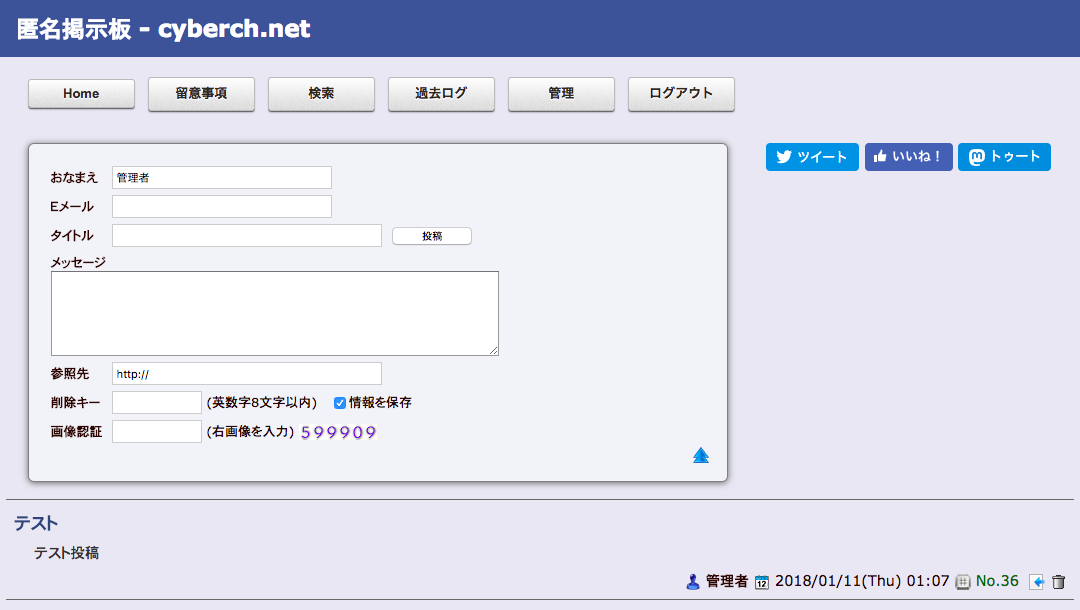
\includegraphics[width=130mm]{figures/bbs_screenshot.png}
	\end{center}
	\caption{匿名掲示板サイト}
	\label{fig: bbs_screenshot}
\end{figure}

掲示板への書込みの際に入力する項目は複数あるが,必須項目は書込みを行った人の名前,書込みのタイトル,本文,画像認証の4項目である.画像認証の項目には,入力欄の右側に画像として表示された数字を入力する.これはスパム投稿を防止するためのものである.先述の通り,名前は実名を入力する必要はないため,個人情報を一切入力せずに投稿できるため,利用者から見ると匿名掲示板のように利用することができる.必須項目を入力して投稿ボタンを押下すると投稿内容がサーバに送信され,書込み一覧に投稿内容が表示される.

\subsection{シェアボタンの設置}
LIGHT BOARDにはシェアボタンは設置されていない.本研究では,SNSのシェアボタンを利用して実験を行うため,シェアボタンを設置した.設置したSNSのシェアボタンは,Twitter,Facebook,Mastodonの3種類である.

Mastodonのシステムは,匿名掲示板サイトと同様に,本研究の実験用に用意したサーバ上に置かれている.そのため,Mastodonのシェアボタンを読み込む際に送信されたCookieは,保存,解析することができる.送信されたCookieを保存し,そのCookieからMastodonのユーザを特定するプログラムを作成した.詳細は後述する.

\subsection{同一ユーザ特定機能の実装}
LIGHT BOARDは,書込み時に名前の入力が必須であるが,同一ユーザが複数の書込みを行う際に,それぞれ異なる名前をつけることが可能である.そのため,複数の書込みが同一人物によるものかどうかを判断することは難しい.そこで,本研究の実験で使用する匿名掲示板には,ユーザを追跡するためのCookieを付与する機能を実装した.

初めて匿名掲示板にアクセスしてきたユーザには,サーバ側で生成したランダムな文字列をCookieとして付与する.2回目以降にアクセスしてきたユーザ(ブラウザ)は,初めてアクセスした際に付与されたCookieをサーバに送信するため,以前にアクセスしたことがあることがサーバ側でわかる.したがって,複数の書込みを行ったユーザは,書込みを行う際に送信しているCookieが同じであるため,同一人物による書込みであることがわかる.

ユーザを追跡するためのCookieを付与する機能に該当する箇所をソースコード\ref{track}に示す.

\begin{lstlisting}[caption=同一ユーザ特定機能,label=track]
use String::Random;

sub track {
  my $host = $ENV{REMOTE_HOST};
  my $addr = $ENV{REMOTE_ADDR};
  my $time = time;
  my ($min,$hour,$mday,$mon,$year,$wday) = (localtime($time))[1..6];
  my @wk = ('Sun','Mon','Tue','Wed','Thu','Fri','Sat');
  my $date = sprintf("%04d/%02d/%02d(%s) %02d:%02d",
        $year+1900,$mon+1,$mday,$wk[$wday],$hour,$min);
  my $cookie = $ENV{HTTP_COOKIE};

  my %cookie;
  foreach (split(/;/, $cookie)) {
    my ($key, $val) = split(/=/);
    $key =~ s/\s//g;
    $cookie{$key} = $val;
  }

  # もしトラッキング用のクッキーがセットされていればファイルに保存する
  # 保存されていなければ新しく発行してセットさせる
  if ($cookie{tracking_id}) {
    open(DAT, ">> $cf{trackingfile}") or error("open err: $cf{trackingfile}");
    my $new = "$date<>$cookie{tracking_id}<>$host<>$addr";
    print DAT "$new\n";
    close(DAT);
  }
  else {
    my $random = String::Random->new();
    my $tracking_id = $random->randregex("[a-zA-Z0-9]{64}");
    print "Set-Cookie: $cf{tracking_id}=$tracking_id\n";
  }
}
\end{lstlisting}

サブルーチンtrackは,トラッキング(特定)用のCookieが送信されなければ新たにCookieを発行し,送信されていればそのCookieをファイルに保存する.発行するCookieは,String::Randomを使用して生成した乱数を値とする.String::Randomを使用して生成する乱数は,大文字,小文字を区別した64文字の英数字であるため,他のユーザと重複する可能性は極めて低いと考えられる.よって,匿名掲示板への書込みとトラッキング用のCookieを照らし合わせ,複数の書込みに対して同じCookieが送信されている場合,同一人物による書込みであると判断できる.

\section{SNS}\label{sec: sns}
本研究では,SNSのアカウントを特定する実験を行うためのシステムとして,Mastodonを利用した.本来のサイバー犯罪においては,TwitterやFacebookなどの,世界的に利用されているSNSの運営と協力して犯人のアカウントを特定することを想定しているが,本研究の実験では,TwitterやFacebookのサーバ内の情報を閲覧することはできない.そこで,個人で運営することができる,Twitterに似たSNSであるMastodonを利用することで,シェアボタンを読み込む際に送信されるCookieからMastodonのアカウントを特定する実験を行った.送信されるCookieからアカウントを特定することは,TwitterやFacebookにおいても技術的に可能であるため,実際のサイバー犯罪ではTwitterやFacebookなどの運営と協力することで,犯人のアカウントが特定できるといえる.

\subsection*{Mastodon}
Mastodonとは,ドイツ人のEugen Rochko氏が,2016年2月に開発を開始した,分散型SNSのことである.Twitterに似た機能を持つSNSとして日本でも注目を集めている.オープンソースソフトウェアとしてGitHub上に公開されており,誰でも自由にプログラムを利用することができる.

TwitterやFacebookとは異なり,Mastodonはプログラムを改変することができ,また改変したプログラムをサーバ上に置いて運営することもできる.Mastodonは分散型SNSであり,個人や団体,企業などが運営するため,複数のサーバが存在する.Mastodonが運営されている各々のサーバのことを,Mastodonのインスタンスと呼ぶ.GitHubからダウンロードしたMastodonのプログラムに,本研究の実験に必要な機能を実装して利用した.

\subsection{シェアボタンの実装}
匿名掲示板に設置するシェアボタンの実装を行った./buttonというURLにアクセスすると,Mastodonのシェアボタンの画像だけが表示されるページを作成した.匿名掲示板では,HTMLのiframeタグを利用し,Mastodonのシェアボタンのページを読み込んでいる.

ユーザ(ブラウザ)は,匿名掲示板にアクセスした際に,Mastodonのシェアボタンを読み込むためにMastodonのサーバにアクセスする.Mastodonのサーバにアクセスする際に,もしユーザがMastodonにログインしている状態であれば,そのログイン状態を保持するCookieをMastodonのサーバに送信するため,匿名掲示板にアクセスしたユーザとMastodonにログインしているユーザを結びつけることができる.

\subsection{送信されたCookieを保存する機能の実装}\label{sec: save_cookie}
匿名掲示板に設置されたシェアボタンを通してMastodonのサーバに送信されたCookieをデータベースに保存する機能を実装した.Mastodonのシェアボタンが読み込まれた際に,送信元の情報を取得し,データベースに保存している.保存する送信元の情報を表\ref{tb: buttons_database}に示す.

\begin{table}[H]
	\caption{保存した送信元のデータ}
	\label{tb: buttons_database}
	\begin{center}
		\begin{tabular}{ | c | c | p{8cm} | } \hline
			データ & データ型 & データ例 \\ \hline
			IPアドレス & string & 133.19.169.6 \\ \hline
			Cookie & text & remember\_user\_token=ABCD1234; \_session\_id=EFGH5678; \_mastodon\_session=IJKL9012  \\ \hline
			リファラ & string & https://www.google.co.jp/ \\ \hline
			ユーザエージェント & string &  Mozilla/5.0 (Macintosh; Intel Mac OS X 10\_12\_6) AppleWebKit/537.36 (KHTML, like Gecko) Chrome/62.0.3202.94 Safari/537.36 \\ \hline
		\end{tabular}
	\end{center}
\end{table}

取得したデータは,IPアドレス,Cookie,リファラ,ユーザエージェントの4つである.データ型は,データベースに保存する際の型を意味する.データ例は,実際に保存されるデータの例を示している.

データベースには,Cookieの他に送信元のIPアドレスやリファラ,ユーザエージェントを保存している.本研究においてはCookieのみの保存で十分であるが,Cookieが取得できなかった場合や,より詳細な情報を得るために,Cookie以外の情報も保存することにした.

\subsection*{リファラ}
リファラとは,どのページからアクセスしたかを示す情報である.例えば,Googleの検索結果からリンクをクリックしてサイトAにアクセスした場合,ブラウザがサイトAに対して送信するリファラはhttps://www.google.co.jp/である.リンクをクリックしてページを遷移した場合に限らず,iframeを使用して別のサイトを読み込んだ場合にもリファラは送信される.匿名掲示板のHTML内に含まれるiframeタグからMastodonのページを読み込んだ場合,Mastodonのサーバに送信されるリファラは,匿名掲示板のURLである.このように,リファラはどのページを経由してアクセスしてきたかがサーバ側にわかるため,Webサイトの解析ツールなどでしばしば用いられる.

\subsection*{ユーザエージェント}
ユーザエージェントとは,ブラウザがサーバに対して送信する情報であり,使用しているブラウザやOS,またその種類などの情報が含まれている.例えば表\ref{tb: buttons_database}のデータ例の場合,アクセスしてきたユーザは,macOS 10.12.6を使用しており,Google Chrome 62.0.3202.94でアクセスしていることがわかる.使用しているブラウザごとにWebページの表示を変えるなど,ユーザビリティの向上を目的に使用されることもあるが,サイバー犯罪においては,犯人の使用しているOSやブラウザがわかるといった利点がある.ただし,ユーザエージェントは詐称(本来とは異なる情報をサーバ側に送信)することも可能であるため,必ずしもユーザエージェントと同じOSやブラウザを使用しているとは限らない.

\subsection{ブラウザフィンガープリンティングの実装}
Cookieやリファラ,ユーザエージェントなどはブラウザからサーバに送信される情報であるが,JavaScriptを使用することで,通常はサーバに送信されない情報を取得することができる.

JavaScriptはブラウザ上で実行されるスクリプト言語であり,Webページの遷移を行うことなくHTMLの構成要素を書き換えたり,非同期でサーバと通信したりすることができる.近年ではほとんどのWebサイトにJavaScriptが使用されている.また,JavaScriptを使用して,ブラウザやデバイスの情報を取得することができる.このように,Cookieの代わりにJavaScriptを利用して,ユーザが使用するデバイスを調べて同一ユーザを特定する仕組みをブラウザフィンガープリンティングという.

ブラウザフィンガープリンティングには,\ref{sec: save_cookie}項で説明したリファラやユーザエージェントなども含まれる.本研究の実験では,通常はサーバに送信されない情報である画面サイズを,JavaScriptを使用して取得することにした.JavaScriptを使用しないと取得できない情報を収集することで,より精度の高い特定手法を提案できると考えられるためである.

サーバ側で,ブラウザから送信された画面サイズの情報を受け取るためのAPIエンドポイントを作成した.APIエンドポイントとは,APIにアクセスする際のURLのことである.本研究では,/api/v1/fingerprintというエンドポイントを作成し,このエンドポイントに対してHTTPのPOSTリクエストが送信された場合に,送信された情報をデータベースに保存する機能を実装した.

JavaScriptでは,ユーザが使用するデバイスの画面サイズを取得し,サーバに送信するプログラムを実装した.該当するJavaScriptのプログラムをソースコード\ref{prog: fingerprint_js}に示す.

\begin{lstlisting}[caption=画面サイズの取得とサーバへの送信,label=prog: fingerprint_js]
var xhr = new XMLHttpRequest();
xhr.open('POST', '/api/v1/fingerprint', true);
xhr.setRequestHeader('content-type', 'application/x-www-form-urlencoded');
xhr.send('screen_size=' + screen.width + 'x' + screen.height);
\end{lstlisting}

JavaScriptでサーバにリクエストを送信する際には,XMLHttpRequest()を使用する.新しく生成したXMLHttpRequest()のオブジェクトを変数xhrに格納する.xhr.open()を使用して,HTTPメソッド(GETやPOSTなど)やリクエストを送信するURL(エンドポイント)を指定する.必要であればxhr.setRequestHeader()を使用してリクエストヘッダを設定することもできる.最後にxhr.send()を使用して,サーバに送信するデータを指定し,送信する.JavaScriptでデバイスの画面サイズを取得するにはscreen.width(画面横幅)とscreen.height(画面縦幅)を使用する.例えばscreen.widthで取得した値が1440,screen.heightで取得した値が900であった場合,'screen\_size=1440x900'という文字列をサーバに送信する.この情報を受け取ったサーバは,データベースにこのデータを文字列として保存する.

\section{実験用ツール}
匿名掲示板とSNSの他に,本研究の実験に当たって必要となるツールの実装を行った.

\subsection{UNIXタイム変換ツール}
匿名掲示板サイトへの書込みは,ファイルに保存するように実装されている.投稿された書込みを保存したファイルの一部を以下に示す.

\begin{verbatim}
5<>2017/12/13(Wed) 18:01<>baz<><>piyo<>ううう<><>133.19.169.6<><>1513155668<>
4<>2017/12/13(Wed) 17:59<>bar<><>huga<>いいい<><>133.19.169.6<><>1513155569<>
3<>2017/12/13(Wed) 17:51<>foo<><>hoge<>あああ<><>133.19.169.6<><>1513155083<>
2<>2017/12/13(Wed) 17:51<>xxx<><>xxx<>test<><>133.19.169.6<><>1513155081<>
1<>2017/12/13(Wed) 17:50<>なまえ<><>無題<>テスト<><>133.19.169.6<><>1513155034<>
\end{verbatim}

投稿された各々の書込みは行ごとに保存されており,書込み内容に関する情報を,\verb|<>|で区切って管理されている.保存されている情報は,左から順に,書込み番号(最初の書込みを1とした連番),投稿時刻,名前,書込みのタイトル,書込みの本文,IPアドレス,UNIXタイムスタンプである.

本研究の実験では,匿名掲示板への書込み時刻とSNSのシェアボタンを読み込む際に送信されたCookieの保存時刻を照合して,書込みを行ったユーザのSNSのアカウントを特定している.書込み内容を管理するファイルには,書込み時刻が保存されているが,秒数までは記録されていない.実際に実験を行ったところ,秒単位でのアクセスが集中したため,書込み時刻からは,Cookieの保存時刻と照合することができなかった.そこで,書込み時刻の代わりにUNIXタイムスタンプを確認することで,Cookieの保存時刻との照合を行った.本研究では,UNIXタイムスタンプを,秒数を含めた時刻に変換するプログラムをPerlで実装した.そのプログラムをソースコード\ref{prog: unix_to_localtime}に示す.

\begin{lstlisting}[caption=UNIXタイムスタンプ変換プログラム,label=prog: unix_to_localtime]
print "localtime: ";
my $num = <STDIN>;
my $time = $num;
my ($sec,$min,$hour,$mday,$mon,$year) = (localtime($time))[0..5];
my $date = sprintf("%04d-%02d-%02d %02d:%02d:%02d",$year+1900,$mon+1,$mday,$hour,$min,$sec);
print "timestamp: " . $date . "\n"
\end{lstlisting}

標準入力からUNIXタイムスタンプを受け取り,時刻に変換して出力するプログラムである.localtime関数は引数として受け取ったUNIXタイムスタンプを9つの要素の配列に変換する関数である\cite{localtime}.ソースコード\ref{prog: unix_to_localtime}では,localtime関数を使用して,入力されたUNIXタイムスタンプから,秒,分,時,日,月,年を取得し,それぞれ変数に格納している.sprintf関数を使用して表示する時刻のフォーマットを指定した後,標準出力を行っている.

\subsection*{UNIXタイムスタンプ}
UNIXタイムスタンプとは,1970年1月1日0時0分0秒を0として,その時刻からの経過秒数を数値で表したものである.たとえば,UNIXタイムスタンプが1513155034であった場合,1970年1月1日0時0分0秒からカウントして1513155034秒が経過した時点での時刻(2017年12月13日17時50分34秒)を表す.ファイルに保存された書込み時刻には秒数が記録されていないが,UNIXタイムスタンプから時刻に変換することで,書き込みがあった時刻の秒数を求めることができる.

\subsection{Railsセッションデコーダ}
本研究の実験に使用するSNSであるMastodonは,Ruby on Rails(以下,Rails)と呼ばれるWebアプリケーションフレームワークを用いて実装されている.Webアプリケーションフレームワークとは,Webアプリケーションにおける一般的な機能を提供する雛形のことである.一般的なWebアプリケーションでは,Webサイトのフォームから入力された情報をデータベースに保存したり,データベースから取得した内容を表示したり,データベースに存在するデータを更新・削除したりする機能がある.それらの機能を,Webアプリケーションの開発者が1から実装することは,開発コストがかかるだけでなく,セキュリティに十分な注意を払わなければ脆弱性を生み出す危険性がある.Webアプリケーションフレームワークを利用すれば,少ない開発コストで,それらの機能を持ったWebアプリケーションを構築することができる.また,多くのWebアプリケーションフレームワークは,オープンソースソフトウェアとしてインターネット上に公開されているため,Webの脆弱性に対する対策が行われている.

ブラウザがWebサービスにログインしている情報は,通常,Cookieに保存されている.ログインに成立すると,サーバはブラウザに,ログイン状態を保持するセッション情報をCookieとして保存するように指示する.以降,セッション情報が含まれるCookieをブラウザがサーバに送信することで,サーバは,アクセスしてきたユーザがログイン済みであると認識する.

したがって,SNSのシステムにおいて,ブラウザから送信されたCookieを調べることで,そのCookieを送信してきたユーザのSNSのアカウントを特定することができる.\ref{sec: sns}節で述べたように,本研究で使用するMastodonに送信されたCookieはデータベースに保存される.ところが,Rails 4.0以降では,セッション情報が暗号化されてCookieに保存されている\cite{rails_session_is_encrypted}ため,そのままではMastodonのアカウントを特定することができない.そこで,データベースに保存されたCookieの中に含まれるセッション情報を複合するプログラムをNode.jsで実装した.そのプログラムをソースコード\ref{prog: rails_session_decoder}に示す.

\begin{lstlisting}[caption=Railsセッションデコーダ,label=prog: rails_session_decoder]
const rsd = require('rails-session-decoder');
const read = require('readline-sync');
const fs = require('fs');

var cookie = read.question('Input your cookie: ');
var key = read.question('Input your secret key: ');

console.log('');

var decoder = rsd(key);

decoder.decodeCookie(cookie, (err, data) => {
  if (data) {
    console.log(data);
  }
  else {
    console.log(err);
  }
});
\end{lstlisting}

暗号化されたセッション情報を復号するには,セッション情報を含むCookieとRails(Mastodon)システム内で管理されている秘密鍵が必要である.セッション情報を含むCookieはデータベースに保存されているものを使用し,秘密鍵はRails(Mastodon)の設定ファイルに書かれているものを使用する.

ソースコード\ref{prog: rails_session_decoder}は,標準入力から,暗号化されたセッション情報を含むCookieと,秘密鍵を受け取り,暗号化されたセッション情報の復号を行う.正しく復号できた場合は復号されたセッション情報を出力し,正しく復号できなかった場合はエラーを出力する.

暗号化されたセッション情報の復号には,rails-session-decoderというNode.jsのパッケージ(ライブラリ)を利用した\cite{npm_rails_session_decoder}.rails-session-decoderを読み取ったオブジェクトに対して,暗号化されたセッション情報を含むCookieと秘密鍵を渡してdecodeCookieメソッドを呼び出すと,暗号化されたセッション情報が復号される.ユーザ(ブラウザ)から送信されたCookieがセッション情報を含んでいれば,復号に成功する.

\newpage






\chapter{実験}
\section{実験内容}
本研究では,SNSのシェアボタンを読み込む際に送信されるCookieから,SNSのアカウントを特定する実験を行った.本実験の目的は,Webサイトに設置されているSNSシェアボタンを利用した,SNSのアカウントの特定可能性を検証するためである.本実験では,TwitterやFacebookに代わるSNSとして,Mastodonを利用した.

本実験を被験者として,立命館大学情報理工学部サイバーセキュリティ研究室に所属する学部生15名に協力を仰いだ.被験者15名には,本研究で用意した匿名掲示板とSNSサイトに対して,以下の事柄を実行してもらった.

\begin{enumerate}
\item{Mastodonアカウントの作成}
\item{メールアドレスの確認とMastodonへのログイン}
\item{匿名掲示板へのアクセス}
\item{匿名掲示板への書込み}
\end{enumerate}

\subsection{Mastodonアカウントの作成}
通常,Mastodonのインスタンスをインターネット上に公開した場合,誰でもそのインスタンスにアカウントを作成することができる.ただし,Mastodon v2.1.0以降では,招待システムが導入され,招待用のリンクを知っている者のみがアカウントを登録することができる\cite{invite_system}.外部の第三者(本実験の被験者ではない者)が,本研究で用意したMastodonインスタンスにアカウントを登録できる状態になっていた場合,本実験で得られるデータの収集の妨げになると判断したため,本研究のMastodonインスタンスでは,招待リンクを知っている者のみがアカウントを登録できるように設定した.事前に招待用のリンクを被験者に配布した.

匿名掲示板へ書込みを行った被験者のMastodonアカウントを特定するため,被験者にはMastodonのアカウントを作成してもらった.アカウント登録ページを図\ref{fig: account_registration}に示す.

\begin{figure}[H]
	\begin{center}
		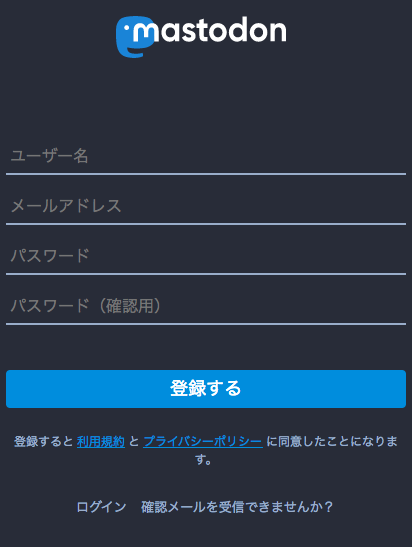
\includegraphics[width=130mm]{figures/account_registration_screenshot.png}
	\end{center}
	\caption{Mastodonアカウント登録ページ}
	\label{fig: account_registration}
\end{figure}

一般的なWebサービスのアカウント登録ページである.被験者は,このフォームにユーザー名(任意の文字列),メールアドレス,パスワードを入力して,アカウントを作成する.

\subsection{メールアドレスの確認とMastodonへのログイン}
アカウントを登録すると,登録時に入力したメールアドレス宛に確認メールが届く.届いたメールに記載されているリンク先にアクセスするとメールアドレスが確認される.登録したアカウントのメールアドレスの有効性が確認できるまで(確認メールのリンク先にアクセスするまで)は,アカウントにログインすることができない.

被験者は,メールアドレスの確認を行った後,ログインページにアクセスしてログインする.

\subsection{匿名掲示板へのアクセス}
被験者は,Mastodonにログインした状態で,匿名掲示板にアクセスする.匿名掲示板もMastodonと同様に,外部から利用されることを防ぐため,アクセス用のパスワードを設置した.アクセス用のパスワードは被験者のみに共有し,第三者から勝手に書込みが行われないようにした.パスワードを入力すると,\ref{sec: bbs}節で示した図\ref{fig: bbs_screenshot}のページが表示される.なお,図\ref{fig: bbs_screenshot}のページにはSNS(Mastodon)のシェアボタンが設置されているため,Mastodonのアカウントにログインした状態でこのページにアクセスした時点で,Mastodonインスタンスにログイン状態を保持するCookieが送信されている.

\subsection{匿名掲示板への書込み}
最後に,被験者は,図\ref{fig: bbs_screenshot}のページから適当な書込みを行う.書き込む際の名前や書込み内容などは,各々の被験者に一任した.また,同一人物が異なる名前で複数の書込みを行っても同一人物による書込みを特定できることを証明するために,一部の被験者には異なる名前で複数の書込みを行ってもらった.

\subsection{匿名掲示板への投稿時の注意点}
匿名掲示板への投稿時に以下の事柄に注意して投稿するよう被験者に説明した.

\begin{itemize}
\item{Mastodonアカウントにログインした状態で投稿すること}
\item{ログインした端末・ブラウザで投稿すること}
\end{itemize}

Mastodonアカウントにログインした状態で書込みを行わなければ,ログイン状態を保持するCookieが送信されないため,アカウントを特定することができない.そのため,被験者には,Mastodonアカウントを作成するだけでなく,作成したアカウントにログインした状態で書込みをするよう指示した.

また,Mastodonアカウントにログインした状態であっても,ログインしたものとは異なる端末・ブラウザを使用して書込みを行った場合も同様に,ログイン状態を保持するCookieが送信されない.そのため,ログインしたものと同じ端末・ブラウザを使用するよう指示した.また,ログインしたものと同じブラウザを使用したとしても,ブラウザのシークレットモード(プライベートブラウジングモード)を使用して書込みを行わないよう指示した.シークレットモードでは,閲覧履歴やCookieがリセットされた状態でブラウジングを行うようになるためである.ただし,シークレットモードでもう一度アカウントにログインし直した場合はこの限りではない.

\section{実験結果}



























% ========== 参考文献 ==========
% 参考文献の引用例(ぶっちゃけ色んな形式があるので後で直せば良さそう)
% \bibitem{引用する番号を付与する際のキーとなる文字列} 著者名(団体名),ウェブサイトの題名 \verb|<URL>| (最終閲覧日: xxxx年xx月xx日)
% \bibitem{test} 特定非営利活動法人デジタル・フォレンジック研究会,デジタルフォレンジックとは \verb|<https://digitalforensic.jp/home/what-df/>| (最終閲覧日: 2015年12月24日)
\begin{thebibliography}{n}
\bibitem{localtime} Japan Perl Association,Perlの組み込み関数 localtime の翻訳 \verb|<http://perldoc.jp/func/localtime>| (最終閲覧日: 2018年1月13日)
\bibitem{rails_session_is_encrypted} Railsのセッション管理方法について \verb|<http://shindolog.hatenablog.com/entry/2014/11/02/164118>| (最終閲覧日: 2018年1月13日)
\bibitem{npm_rails_session_decoder} rails-session-decoder \verb|<https://www.npmjs.com/package/rails-session-decoder>| (最終閲覧日: 2018年1月13日)
\bibitem{invite_system} Release v2.1.0 \UTF{00B7} tootsuite/mastodon \verb|<https://github.com/tootsuite/mastodon/releases/tag/v2.1.0>| (最終閲覧日: 2018年1月14日)

\end{thebibliography}
% ============================





\begin{comment}
表の挿入はここから
\begin{table}[H]
	\caption{表のタイトルを入力}
	\label{tb: example1}
	\begin{center}
		\begin{tabular}{ | c | c | c | } \hline
			タイトル & タイトル & タイトル \\ \hline\hline
			内容1-1 & 内容1-2 & 内容1-3 \\ \hline
			内容2-1 & 内容2-2 & 内容2-3 \\ \hline
		\end{tabular}
	\end{center}
\end{table}
表の挿入はここまで
表\ref{tb: example1}のように表番号を参照することができます.
\end{comment}

\begin{comment}
図の挿入はここから
\begin{figure}[H]
	\begin{center}
		\includegraphics[width=(好きな数値)mm]{画像ファイル名を入力}
	\end{center}
	\caption{図のタイトルを入力}
	\label{fig: example1}
\end{figure}
図の挿入はここまで
図\ref{fig: example1}のように図番号を参照することができます.
\end{comment}





\end{document}